\documentclass[11pt,a4paper]{report}
\usepackage[textwidth=37em,vmargin=30mm]{geometry}
\usepackage{calc,xunicode,amsmath,amssymb,paralist,enumitem,tabu,booktabs,datetime2,xeCJK,xeCJKfntef,listings}
\usepackage{tocloft,fancyhdr,tcolorbox,xcolor,graphicx,eso-pic,xltxtra,xelatexemoji}

\newcommand{\envyear}[0]{2025}
\newcommand{\envdatestr}[0]{2025-03-31}
\newcommand{\envfinaldir}[0]{webdb/2025/20250331/final}

\usepackage[hidelinks]{hyperref}
\hypersetup{
    colorlinks=false,
    pdfpagemode=FullScreen,
    pdftitle={Web Digest - \envdatestr}
}

\setlength{\cftbeforechapskip}{10pt}
\renewcommand{\cftchapfont}{\rmfamily\bfseries\large\raggedright}
\setlength{\cftbeforesecskip}{2pt}
\renewcommand{\cftsecfont}{\sffamily\small\raggedright}

\setdefaultleftmargin{2em}{2em}{1em}{1em}{1em}{1em}

\usepackage{xeCJK,xeCJKfntef}
\xeCJKsetup{PunctStyle=plain,RubberPunctSkip=false,CJKglue=\strut\hskip 0pt plus 0.1em minus 0.05em,CJKecglue=\strut\hskip 0.22em plus 0.2em}
\XeTeXlinebreaklocale "zh"
\XeTeXlinebreakskip = 0pt


\setmainfont{Brygada 1918}
\setromanfont{Brygada 1918}
\setsansfont{IBM Plex Sans}
\setmonofont{JetBrains Mono NL}
\setCJKmainfont{Noto Serif CJK SC}
\setCJKromanfont{Noto Serif CJK SC}
\setCJKsansfont{Noto Sans CJK SC}
\setCJKmonofont{Noto Sans CJK SC}

\setlength{\parindent}{0pt}
\setlength{\parskip}{8pt}
\linespread{1.15}

\lstset{
	basicstyle=\ttfamily\footnotesize,
	numbersep=5pt,
	backgroundcolor=\color{black!5},
	showspaces=false,
	showstringspaces=false,
	showtabs=false,
	tabsize=2,
	captionpos=b,
	breaklines=true,
	breakatwhitespace=true,
	breakautoindent=true,
	linewidth=\textwidth
}






\newcommand{\coverpic}[2]{
    % argv: itemurl, authorname
    Cover photo by #2~~(\href{#1}{#1})
}
\newcommand{\makeheader}[0]{
    \begin{titlepage}
        % \newgeometry{hmargin=15mm,tmargin=21mm,bmargin=12mm}
        \begin{center}
            
            \rmfamily\scshape
            \fontspec{BaskervilleF}
            \fontspec{Old Standard}
            \fontsize{59pt}{70pt}\selectfont
            WEB\hfill DIGEST
            
            \vfill
            % \vskip 30pt
            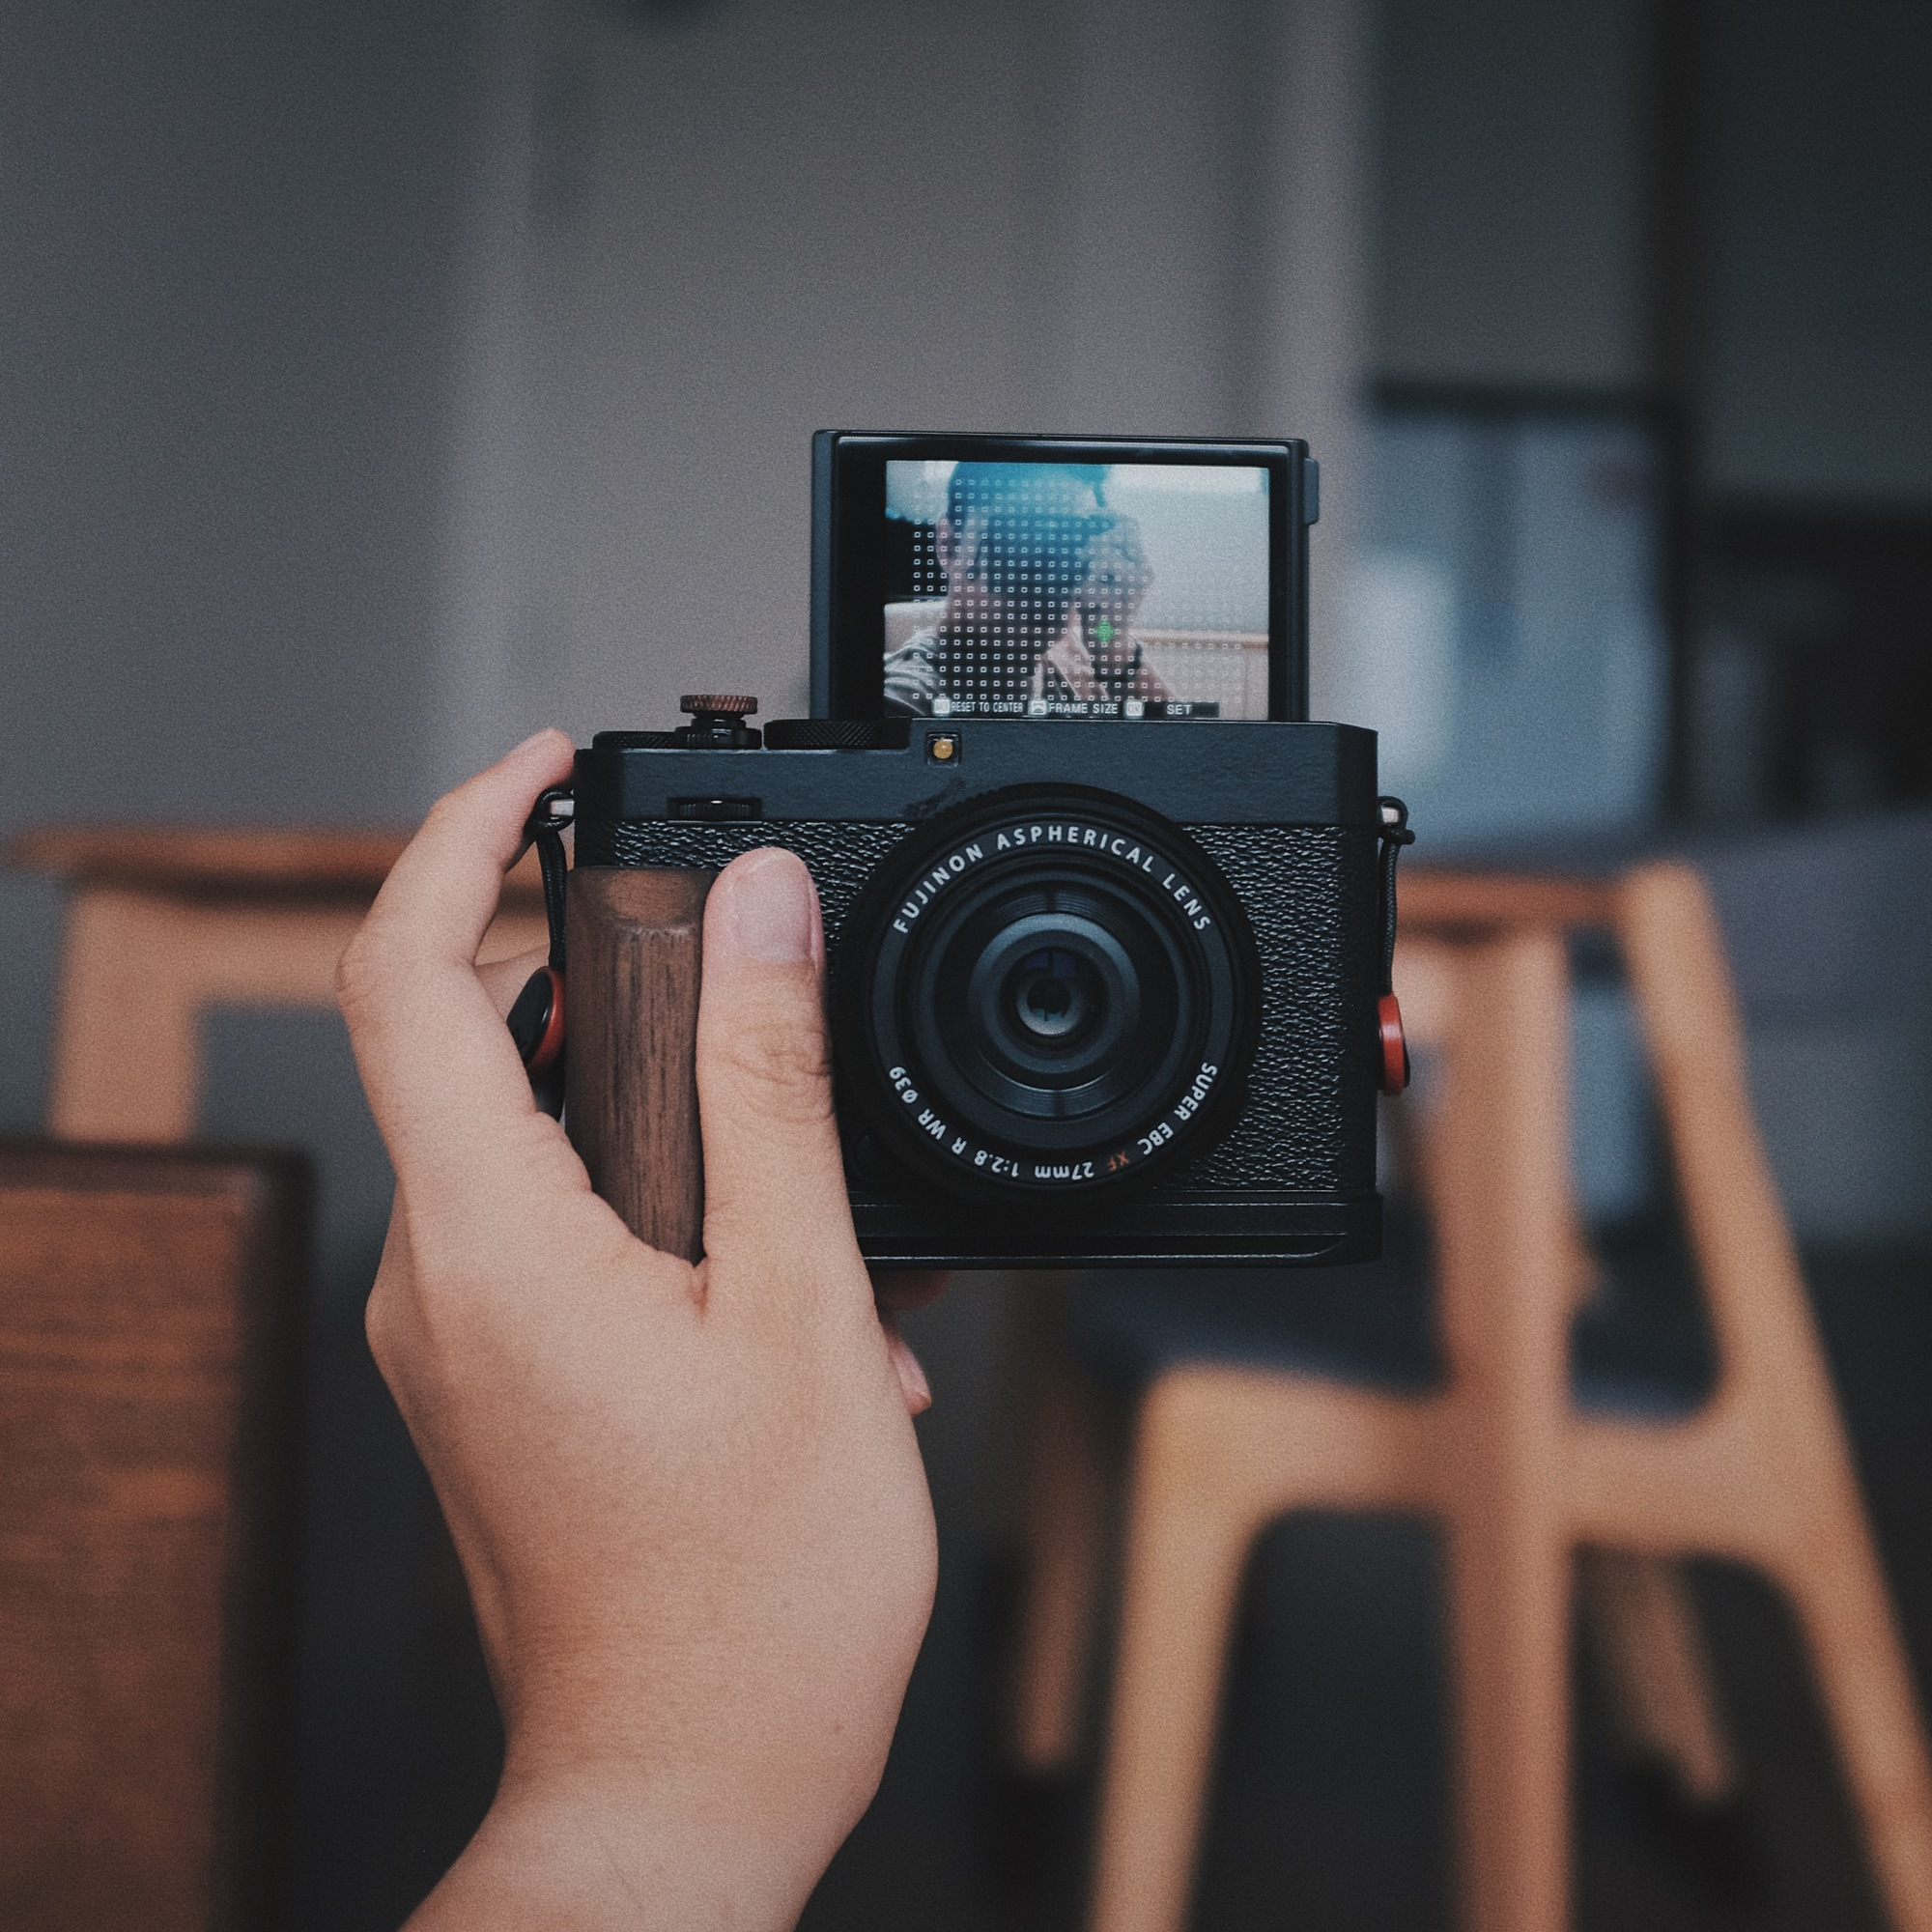
\includegraphics[width=\linewidth]{\envfinaldir/coverpic-prod.jpg}\par
            % \vskip 30pt
            \vfill

            \normalsize\rmfamily\scshape
            \copyright{} The Web Digest Project \hfill\large \envdatestr
        \end{center}
    \end{titlepage}
    % \restoregeometry
}
\newcommand{\simplehref}[1]{%
    \textcolor{blue!80!green}{\href{#1}{#1}}%
}
\renewcommand{\contentsname}{\center\Huge\sffamily\bfseries Contents\par\vskip 20pt}
\newcounter{ipartcounter}
\setcounter{ipartcounter}{0}
\newcommand{\ipart}[1]{
    % \vskip 20pt
    \clearpage
    \stepcounter{ipartcounter}
    \phantomsection
    \addcontentsline{toc}{chapter}{#1}
    % \begin{center}
    %     \Huge
    %     \sffamily\bfseries
    %     #1
    % \end{center}
    % \vskip 20pt plus 7pt
}
\newcounter{ichaptercounter}
\setcounter{ichaptercounter}{0}
\newcommand{\ichapter}[1]{
    % \vskip 20pt
    \clearpage
    \stepcounter{ichaptercounter}
    \phantomsection
    \addcontentsline{toc}{section}{\numberline{\arabic{ichaptercounter}}#1}
    \begin{center}
        \Huge
        \sffamily\bfseries
        #1
    \end{center}
    \vskip 20pt plus 7pt
}
\newcommand{\entrytitlefont}[1]{\subsection*{\raggedright\Large\sffamily\bfseries#1}}
\newcommand{\entryitemGeneric}[2]{
    % argv: title, url
    \parbox{\linewidth}{
        \entrytitlefont{#1}\par\vskip 5pt
        \footnotesize\ttfamily\mdseries
        \simplehref{#2}
    }\vskip 11pt plus 11pt minus 1pt
}
\newcommand{\entryitemGithub}[3]{
    % argv: title, url, desc
    \parbox{\linewidth}{
        \entrytitlefont{#1}\par\vskip 5pt
        \footnotesize\ttfamily\mdseries
        \simplehref{#2}\par\vskip 5pt
        \small\rmfamily\mdseries#3
    }\vskip 11pt plus 11pt minus 1pt
}
\newcommand{\entryitemAp}[3]{
    % argv: title, url, desc
    \parbox{\linewidth}{
        \entrytitlefont{#1}\par\vskip 5pt
        \footnotesize\ttfamily\mdseries
        \simplehref{#2}\par\vskip 5pt
        \small\rmfamily\mdseries#3
    }\vskip 11pt plus 11pt minus 1pt
}
\newcommand{\entryitemHackernews}[3]{
    % argv: title, hnurl, rawurl
    % \parbox{\linewidth}{
    %     \entrytitlefont{#1}\par\vskip 5pt
    %     \footnotesize\ttfamily\mdseries
    %     \simplehref{#3}\par
    %     \textcolor{black!50}{\href{#2}{#2}}
    % }\vskip 11pt plus 11pt minus 1pt
    \begin{minipage}{\linewidth}
            \entrytitlefont{#1}\par\vskip 5pt
            \footnotesize\ttfamily\mdseries
            \simplehref{#3}\par
            \textcolor{black!50}{\href{#2}{#2}}
    \end{minipage}\par\vskip 11pt plus 11pt minus 1pt
}







\begin{document}

\makeheader

\tableofcontents\clearpage




\ipart{Developers}
\ichapter{Hacker News}
\entryitemTwoLinks{ICE Arrested and Detained a US Citizen for Hours Because He Looked Mexican}{https://news.ycombinator.com/item?id=43527275}{https://www.techdirt.com/2025/03/28/ice-arrested-and-detained-a-us-citizen-for-hours-because-he-looked-mexican/}

\entryitemTwoLinks{Man Detained by ICE for Autism Awareness Tattoo Sent to Prison}{https://news.ycombinator.com/item?id=43527154}{https://www.latintimes.com/man-detained-ice-autism-awareness-tattoo-still-sent-prison-after-officers-declared-him-clean-579373}

\entryitemTwoLinks{Public secrets exposure leads to supply chain attack on GitHub CodeQL}{https://news.ycombinator.com/item?id=43527044}{https://www.praetorian.com/blog/codeqleaked-public-secrets-exposure-leads-to-supply-chain-attack-on-github-codeql/}

\entryitemTwoLinks{FBI raids home of prominent computer scientist who has gone incommunicado}{https://news.ycombinator.com/item?id=43527001}{https://arstechnica.com/security/2025/03/computer-scientist-goes-silent-after-fbi-raid-and-purging-from-university-website/}

\entryitemTwoLinks{Met Police smash down door of Quaker meeting house to arrest activists}{https://news.ycombinator.com/item?id=43525909}{https://www.thetimes.com/uk/society/article/met-smash-down-door-of-quaker-meeting-house-to-arrest-activists-jhhchrtlt}

\entryitemTwoLinks{Blue95: a desktop for your childhood home's computer room}{https://news.ycombinator.com/item?id=43524937}{https://github.com/winblues/blue95}

\entryitemTwoLinks{Span<T>.SequenceEquals is faster than memcmp}{https://news.ycombinator.com/item?id=43524665}{https://richardcocks.github.io/2025-03-30-FasterThanMemCmp.html}

\entryitemTwoLinks{Hacker Laws}{https://news.ycombinator.com/item?id=43523974}{https://hacker-laws.com/}

\entryitemTwoLinks{Rust Any part 3: we have upcasts}{https://news.ycombinator.com/item?id=43523238}{https://lucumr.pocoo.org/2025/3/27/any-upcast/}

\entryitemTwoLinks{The average college student today}{https://news.ycombinator.com/item?id=43522966}{https://hilariusbookbinder.substack.com/p/the-average-college-student-today}

\entryitemTwoLinks{Four Lectures on Standard ML (1989) [pdf]}{https://news.ycombinator.com/item?id=43522363}{https://www.cs.tufts.edu/~nr/cs257/archive/mads-tofte/four-lectures.pdf}

\entryitemTwoLinks{Show HN: Cloud-Ready Postgres MCP Server}{https://news.ycombinator.com/item?id=43520953}{https://github.com/stuzero/pg-mcp}

\entryitemTwoLinks{My TV started playing a video in full screen by itself. What happened?}{https://news.ycombinator.com/item?id=43520074}{https://support.vizio.com/s/article/Ambient-or-Scenic-Mode-showing-on-my-TV?language=en\_US}

\entryitemTwoLinks{Buy once, use forever A directory of one-time purchase software}{https://news.ycombinator.com/item?id=43519998}{https://buyoncesoftware.com/}

\entryitemTwoLinks{Trump's Police Are Now Disappearing Students for Their Op-Eds}{https://news.ycombinator.com/item?id=43519864}{https://www.techdirt.com/2025/03/27/trumps-secret-police-are-now-disappearing-students-for-their-op-eds/}

\entryitemTwoLinks{Towards fearless SIMD, 7 years later}{https://news.ycombinator.com/item?id=43519823}{https://linebender.org/blog/towards-fearless-simd/}

\entryitemTwoLinks{Self-contained Python scripts with uv}{https://news.ycombinator.com/item?id=43519669}{http://blog.dusktreader.dev/2025/03/29/self-contained-python-scripts-with-uv/}

\entryitemTwoLinks{Convert Linux to Windows}{https://news.ycombinator.com/item?id=43518917}{https://philipbohun.com/blog/0007.html}

\entryitemTwoLinks{Everyone knows all the apps on your phone}{https://news.ycombinator.com/item?id=43518866}{https://peabee.substack.com/p/everyone-knows-what-apps-you-use}

\entryitemTwoLinks{Apple's AI isn't a letdown. AI is the letdown}{https://news.ycombinator.com/item?id=43518576}{https://www.cnn.com/2025/03/27/tech/apple-ai-artificial-intelligence/index.html}\ichapter{Phoronix}
\entryitemGeneric{\hskip 0pt{}CachyOS Adds Limine Bootloader, Easier Samba Integration \& NTSYNC Wine}{https://www.phoronix.com/news/CachyOS-March-2025-Release}

\entryitemGeneric{\hskip 0pt{}Chromium Web Browser Lands Support For Wayland XDG-Session-Management}{https://www.phoronix.com/news/Chrome-XDG-Session-Management}

\entryitemGeneric{\hskip 0pt{}IO\_uring Network Zero-Copy Receive Lands In Linux 6.15}{https://www.phoronix.com/news/Linux-6.15-IO\_uring}

\entryitemGeneric{\hskip 0pt{}Lenovo ThinkEdge SE30 Watchdog Driver Coming For Linux 6.15}{https://www.phoronix.com/news/Linux-6.15-Watchdog}

\entryitemGeneric{\hskip 0pt{}Mesa's Exciting Q1 With More Ray-Tracing, NVK Progress \& Performance Optimizations}{https://www.phoronix.com/news/Mesa-Q1-2025-Highlights}

\entryitemGeneric{\hskip 0pt{}MIPS Lands Multi-Cluster Support In Linux 6.15 For The EyeQ6 SoC}{https://www.phoronix.com/news/Linux-6.15-MIPS}

\entryitemGeneric{\hskip 0pt{}Shotcut 25.03 Open-Source, Cross-Platform Video Editor Released}{https://www.phoronix.com/news/Shotcut-25.03-Released}

\entryitemGeneric{\hskip 0pt{}Intel's 2025-Q1 Linux Excitement With Battlemage, AVX10 \& Other Kernel Improvements}{https://www.phoronix.com/news/Intel-Linux-2025-Q1-Recap}

\entryitemGeneric{\hskip 0pt{}Firmware Loader Makes It Possible To Use Old Samsung TV Cameras On Linux}{https://www.phoronix.com/news/Samsung-TV-Cameras-Linux}\ichapter{Dribbble}
\entryitemGeneric{\hskip 0pt{}I'm leaving Dribbble. After 15 years.}{https://dribbble.com/shots/25836899-I-m-leaving-Dribbble-After-15-years}

\entryitemGeneric{\hskip 0pt{}The Rocky token landing page}{https://dribbble.com/shots/25827682-The-Rocky-token-landing-page}

\entryitemGeneric{\hskip 0pt{}Banking Mobile App Design}{https://dribbble.com/shots/25829959-Banking-Mobile-App-Design}

\entryitemGeneric{\hskip 0pt{}Big gestures}{https://dribbble.com/shots/25826632-Big-gestures}

\entryitemGeneric{\hskip 0pt{}Proven UI/UX design, User Interface experience}{https://dribbble.com/shots/25819444-Proven-UI-UX-design-User-Interface-experience}

\entryitemGeneric{\hskip 0pt{}Dog + Play Button}{https://dribbble.com/shots/25809362-Dog-Play-Button}

\entryitemGeneric{\hskip 0pt{}Pricefy Logo Design - Mountains, Chart, Graph, Sun}{https://dribbble.com/shots/25824720-Pricefy-Logo-Design-Mountains-Chart-Graph-Sun}

\entryitemGeneric{\hskip 0pt{}Illustration}{https://dribbble.com/shots/25822720-Illustration}

\entryitemGeneric{\hskip 0pt{}Crypto Portfolio Tracker App}{https://dribbble.com/shots/25820014-Crypto-Portfolio-Tracker-App}

\entryitemGeneric{\hskip 0pt{}Gemini Rebrand}{https://dribbble.com/shots/25821410-Gemini-Rebrand}

\entryitemGeneric{\hskip 0pt{}Cyber Extrusion (Merch/Custom T-shirt)}{https://dribbble.com/shots/25821987-Cyber-Extrusion-Merch-Custom-T-shirt}

\entryitemGeneric{\hskip 0pt{}FCKD - Part 2}{https://dribbble.com/shots/25817864-FCKD-Part-2}

\entryitemGeneric{\hskip 0pt{}ROOT BEER}{https://dribbble.com/shots/25815759-ROOT-BEER}

\entryitemGeneric{\hskip 0pt{}Aura - Logo Design}{https://dribbble.com/shots/25815819-Aura-Logo-Design}

\entryitemGeneric{\hskip 0pt{}Complexure}{https://dribbble.com/shots/25815646-Complexure}

\entryitemGeneric{\hskip 0pt{}Snitcher - New Branding}{https://dribbble.com/shots/25816140-Snitcher-New-Branding}

\entryitemGeneric{\hskip 0pt{}Lepisov Branding Logo Reveal Animation}{https://dribbble.com/shots/25814536-Lepisov-Branding-Logo-Reveal-Animation}

\entryitemGeneric{\hskip 0pt{}Spark illustrations}{https://dribbble.com/shots/25815705-Spark-illustrations}

\entryitemGeneric{\hskip 0pt{}FCKD}{https://dribbble.com/shots/25812257-FCKD}

\entryitemGeneric{\hskip 0pt{}Spark}{https://dribbble.com/shots/25815686-Spark}

\entryitemGeneric{\hskip 0pt{}Revobyte Logo Design - R Letter / Monogram / Blockchain}{https://dribbble.com/shots/25811483-Revobyte-Logo-Design-R-Letter-Monogram-Blockchain}

\entryitemGeneric{\hskip 0pt{}Spark illustrations}{https://dribbble.com/shots/25815717-Spark-illustrations}

\entryitemGeneric{\hskip 0pt{}S}{https://dribbble.com/shots/25814436-S}

\entryitemGeneric{\hskip 0pt{}Cimet Merch Car Wrapp}{https://dribbble.com/shots/25710572-Cimet-Merch-Car-Wrapp}


\ipart{Developers~~~~(zh-Hans)}
\ichapter{Solidot}
\entryitemGeneric{\hskip 0pt{}火星尘埃可能会对宇航员构成健康威胁}{https://www.solidot.org/story?sid=80921}

\entryitemGeneric{\hskip 0pt{}法航因乘客手机丢失而被迫返航}{https://www.solidot.org/story?sid=80920}

\entryitemGeneric{\hskip 0pt{}科学家可能找到了阻止秃顶的方法}{https://www.solidot.org/story?sid=80919}

\entryitemGeneric{\hskip 0pt{}天文学家首度确认海王星存在极光现象}{https://www.solidot.org/story?sid=80918}

\entryitemGeneric{\hskip 0pt{}未来的 Windows 版本将必须要有网络连接和 Microsoft Account 账号才能安装}{https://www.solidot.org/story?sid=80917}

\entryitemGeneric{\hskip 0pt{}涉及 Waymos 的绝大多数车祸都是人类司机引起的}{https://www.solidot.org/story?sid=80916}

\entryitemGeneric{\hskip 0pt{}AI 数据中心太多了}{https://www.solidot.org/story?sid=80915}

\entryitemGeneric{\hskip 0pt{}哥伦比亚大学学生因 AI 面试编程作弊工具而被停学}{https://www.solidot.org/story?sid=80914}

\entryitemGeneric{\hskip 0pt{}Ubuntu 25.04 (Plucky Puffin) Beta 释出}{https://www.solidot.org/story?sid=80913}

\entryitemGeneric{\hskip 0pt{}微软用预加载加速 Microsoft Office 启动}{https://www.solidot.org/story?sid=80912}

\entryitemGeneric{\hskip 0pt{}数据揭示了佛罗里达州在超速驾驶执法中存在种族歧视}{https://www.solidot.org/story?sid=80911}

\entryitemGeneric{\hskip 0pt{}缅甸发生 7.9 级/M7.7 级地震}{https://www.solidot.org/story?sid=80910}

\entryitemGeneric{\hskip 0pt{}吉卜力风格 AI 图像引版权争议}{https://www.solidot.org/story?sid=80909}

\entryitemGeneric{\hskip 0pt{}马的非凡耐力来自其基因突变}{https://www.solidot.org/story?sid=80908}

\entryitemGeneric{\hskip 0pt{}马斯克施压 Reddit CEO 去压制对其及 DOGE 的批评}{https://www.solidot.org/story?sid=80907}

\entryitemGeneric{\hskip 0pt{}Signal 在美国和也门的下载量大幅飙升}{https://www.solidot.org/story?sid=80906}

\entryitemGeneric{\hskip 0pt{}腾讯向育碧子公司投资 11.6 亿欧元}{https://www.solidot.org/story?sid=80905}

\entryitemGeneric{\hskip 0pt{}Valve 证实 Steam 简体中文玩家超过英语玩家}{https://www.solidot.org/story?sid=80904}\ichapter{V2EX}
\entryitemGeneric{\hskip 0pt{}[程序员] 对程序员来说,不需要给 AI 付费编程}{https://www.v2ex.com/t/1122152}

\entryitemGeneric{\hskip 0pt{}[问与答] 豆包的语音对话做的真好, 但是 AI 很一般}{https://www.v2ex.com/t/1122150}

\entryitemGeneric{\hskip 0pt{}[问与答] gemini2.5pro 编程能力怎么样有人试过吗}{https://www.v2ex.com/t/1122149}

\entryitemGeneric{\hskip 0pt{}[程序员] 新人跳槽求指导}{https://www.v2ex.com/t/1122148}

\entryitemGeneric{\hskip 0pt{}[macOS] macOS 15.4 是否将 IDEA IDE 干碎?}{https://www.v2ex.com/t/1122147}

\entryitemGeneric{\hskip 0pt{}[分享创造] 4090 显卡,基于 Flux 造了个 100\%免费,不限量的 AI 生成工具,代替 Stable Diffusion 和 Midjourney}{https://www.v2ex.com/t/1122146}

\entryitemGeneric{\hskip 0pt{}[推广] 「回血计划」无需存量证明的券商,开户额外返 150hkd}{https://www.v2ex.com/t/1122145}

\entryitemGeneric{\hskip 0pt{}[问与答] 大佬们都是怎么推广自己的开源项目}{https://www.v2ex.com/t/1122144}

\entryitemGeneric{\hskip 0pt{}[随想] 好快啊!又是一年清明节!}{https://www.v2ex.com/t/1122143}

\entryitemGeneric{\hskip 0pt{}[宽带症候群] 有没有人抓一下陕西(西安)联通 IPTV}{https://www.v2ex.com/t/1122142}

\entryitemGeneric{\hskip 0pt{}[问与答] 抖音直播改变了传输格式,导致直播视频无法播放}{https://www.v2ex.com/t/1122141}

\entryitemGeneric{\hskip 0pt{}[问与答] 23 年毕业二本,数控 qt+图像处理工程师。东莞月薪 9k,求助各位大佬未来有什么发展方向推荐。}{https://www.v2ex.com/t/1122140}

\entryitemGeneric{\hskip 0pt{}[分享创造] 做了个专门背后阴阳领导的表情包生成器}{https://www.v2ex.com/t/1122138}

\entryitemGeneric{\hskip 0pt{}[问与答] W11 风扇呼呼转, 一打开任务管理器 cpu 占用率就慢慢 降低下来了, 啥情况这是?}{https://www.v2ex.com/t/1122137}

\entryitemGeneric{\hskip 0pt{}[问与答] 大家觉得 35k 以上的 goer 需要哪些技能}{https://www.v2ex.com/t/1122135}

\entryitemGeneric{\hskip 0pt{}[分享创造] 我开发了一个在线转换 unix 时间戳 timestamp 日期格式的网站 timestamp.onl}{https://www.v2ex.com/t/1122134}

\entryitemGeneric{\hskip 0pt{}[DNS] 教育网 DNS 对 cloudflare 的 tunnel 隧道建站的 dns 查询支持不好吗}{https://www.v2ex.com/t/1122132}

\entryitemGeneric{\hskip 0pt{}[程序员] Cursor 的 500 次用完是重新搞个号注册 Pro 还是用 Api 的?}{https://www.v2ex.com/t/1122131}

\entryitemGeneric{\hskip 0pt{}[问与答] 如何让 macOS Finder 显示真正的最近文件和最近文件夹?}{https://www.v2ex.com/t/1122130}

\entryitemGeneric{\hskip 0pt{}[Android] 已 root,改定位用什么好, fake location 强制更新收费太难受了}{https://www.v2ex.com/t/1122128}

\entryitemGeneric{\hskip 0pt{}[问与答] 有没有做过 app 运营推广的朋友?}{https://www.v2ex.com/t/1122127}

\entryitemGeneric{\hskip 0pt{}[奇思妙想] 搞了一个都是猫猫游戏的合集 cat-game.online}{https://www.v2ex.com/t/1122124}

\entryitemGeneric{\hskip 0pt{}[Apple TV] 求推荐局域网播放软件}{https://www.v2ex.com/t/1122122}

\entryitemGeneric{\hskip 0pt{}[问与答] Grok 镜像网站疑问}{https://www.v2ex.com/t/1122121}

\entryitemGeneric{\hskip 0pt{}[问与答] 父亲生病,我该不该辞职?}{https://www.v2ex.com/t/1122120}

\entryitemGeneric{\hskip 0pt{}[问与答] 有什么好的办法解决微服务项目运行, cpu 过高问题?}{https://www.v2ex.com/t/1122117}

\entryitemGeneric{\hskip 0pt{}[摄影] 大疆 mini3pro 可以去云南或者大西北吗}{https://www.v2ex.com/t/1122116}

\entryitemGeneric{\hskip 0pt{}[Apple] 我一直觉得新款 MPB 变重了,果然。}{https://www.v2ex.com/t/1122115}

\entryitemGeneric{\hskip 0pt{}[分享创造] [分享] Ghibli AI 工具 - 免费将照片转换为吉卜力动画风格 | GhibliAI.tools}{https://www.v2ex.com/t/1122113}

\entryitemGeneric{\hskip 0pt{}[分享创造] 开发了一款跨平台的下载工具,兄弟们可以给个 star 吗?有兴趣的一起来维护啊 c++ 搞的}{https://www.v2ex.com/t/1122111}

\entryitemGeneric{\hskip 0pt{}[问与答] AI 产品 创意集}{https://www.v2ex.com/t/1122110}

\entryitemGeneric{\hskip 0pt{}[问与答] 不知道为什么这块磁盘会导致,主板无法进入 BOIS 设置界面}{https://www.v2ex.com/t/1122107}

\entryitemGeneric{\hskip 0pt{}[奇思妙想] 来探索你的网络人格试试(非常犀利)}{https://www.v2ex.com/t/1122106}

\entryitemGeneric{\hskip 0pt{}[Edge] edge browser 的 window.outerWidth 和 window.innerWidth 不一样}{https://www.v2ex.com/t/1122105}

\entryitemGeneric{\hskip 0pt{}[NAS] 求个 nas 上能用的同步备份工具}{https://www.v2ex.com/t/1122102}

\entryitemGeneric{\hskip 0pt{}[问与答] 翻译模型哪家强?}{https://www.v2ex.com/t/1122101}

\entryitemGeneric{\hskip 0pt{}[OpenAI] Anthropic 还有 \$ 3 API 余额, 4 月 15 日到期, V 友们谁有需要就拿去用吧}{https://www.v2ex.com/t/1122100}

\entryitemGeneric{\hskip 0pt{}[宽带症候群] 我发现代理客户端喜欢自己实现一遍协议}{https://www.v2ex.com/t/1122099}

\entryitemGeneric{\hskip 0pt{}[程序员] 如何交互式多进程执行 shell 脚本中的所有命令?}{https://www.v2ex.com/t/1122098}

\entryitemGeneric{\hskip 0pt{}[机械键盘] 三模 87 键盘推荐}{https://www.v2ex.com/t/1122097}

\entryitemGeneric{\hskip 0pt{}[开源软件] 写了一个 opensearch 的 dify 插件,欢迎围观}{https://www.v2ex.com/t/1122096}

\entryitemGeneric{\hskip 0pt{}[分享发现] 大家有什么年度博文、方法或者工具推荐}{https://www.v2ex.com/t/1122095}

\entryitemGeneric{\hskip 0pt{}[问与答] 微信支付的金币 怎么没活动了,攒了 100 多个}{https://www.v2ex.com/t/1122094}

\entryitemGeneric{\hskip 0pt{}[分享创造] 真正的 AI 赋能 RAW 修图}{https://www.v2ex.com/t/1122093}

\entryitemGeneric{\hskip 0pt{}[程序员] 在家里用公司的电脑干个人项目,风险大吗?}{https://www.v2ex.com/t/1122092}

\entryitemGeneric{\hskip 0pt{}[分享创造] Lazyapi 通过终端管理你的 API}{https://www.v2ex.com/t/1122091}

\entryitemGeneric{\hskip 0pt{}[Windows] 无语了, win 的蓝牙 wifi 功能窗关不了}{https://www.v2ex.com/t/1122089}

\entryitemGeneric{\hskip 0pt{}[奇思妙想] 咨询 如果有一个智能报价系统,大家会使用吗?}{https://www.v2ex.com/t/1122087}

\entryitemGeneric{\hskip 0pt{}[问与答] 14 寸不要求游戏性能的笔记本电脑,排除苹果联想 HP 华为以及小众品牌还能剩下几个牌子能买}{https://www.v2ex.com/t/1122086}

\entryitemGeneric{\hskip 0pt{}[无人机] mini3pro 可以去云南或者大西北吗}{https://www.v2ex.com/t/1122085}


\ipart{Generic News}
\ichapter{AP News}
\entryitemWithDescription{\hskip 0pt{}Historic tree to be cut down at the White House over safety concerns}{https://apnews.com/article/21d3f53568bf5f9c64050a2732c034c6}{}

\entryitemWithDescription{\hskip 0pt{}First disappointment and then a celebration as video captures high school band's big surprise}{https://apnews.com/article/b600817b366c995b53027da348992eed}{}

\entryitemWithDescription{\hskip 0pt{}Statham's `A Working Man' upsets `Snow White' to take No. 1 at the box office}{https://apnews.com/article/c1cb5cec29c2278cd23c08935ca4531d}{}

\entryitemWithDescription{\hskip 0pt{}Chair of African charity Prince Harry co-founded says he orchestrated a bullying campaign}{https://apnews.com/article/c8adbbb632fe6a7fa765bf6781395104}{}

\entryitemWithDescription{\hskip 0pt{}Tsunami warning lifted after 7.0 earthquake near Tonga in the South Pacific}{https://apnews.com/article/0bcaab5e5e83156846a65ed46556391e}{}

\entryitemWithDescription{\hskip 0pt{}Doctor cites the pope's `surprising improvement' after surviving life-threatening crises}{https://apnews.com/article/7fa0d692e3ba1a94ca936101a28dbe26}{}

\entryitemWithDescription{\hskip 0pt{}Venice says it will host Bezos wedding and denies reports of possible disruptions for the city}{https://apnews.com/article/375cc08aed84871693303347e27ebe84}{}

\entryitemWithDescription{\hskip 0pt{}Judge homers 3 times as Yanks go deep on Cortes' first 3 pitches and hit 9 HRs vs. Brewers}{https://apnews.com/article/0af6773313e0ccd0bfba5933eee628b3}{}

\entryitemWithDescription{\hskip 0pt{}`Wellness rooms' are claiming space in many homes}{https://apnews.com/article/fc6d0df76284dbc569c8032e2126791d}{}

\entryitemWithDescription{\hskip 0pt{}Passenger flight and Air Force jet diverted from potential collision at DC airport}{https://apnews.com/article/888e2dd4e9c9d6506a37e9e6a24cfe17}{}

\entryitemWithDescription{\hskip 0pt{}Richard Chamberlain, TV actor who starred in `Dr. Kildare,' dies at 90}{https://apnews.com/article/12771b3863b74c3eb5806e4ba33de445}{}

\entryitemWithDescription{\hskip 0pt{}Ring bling: Dodgers show off glittering World Series rings in pregame ceremony}{https://apnews.com/article/445edc192a392f9d1fa012d5a14ef181}{}

\entryitemWithDescription{\hskip 0pt{}Cuba had record 26 players on opening-day MLB rosters and Japan had 12 for its most since 2012}{https://apnews.com/article/ab72db7526b38b7f8a70474cc2f6e398}{}\ichapter{Reuters}
\entryitemWithDescription{\hskip 0pt{}Israel strikes Lebanon in response to cross-border rocket fire}{https://www.reuters.com/world/middle-east/israel-strikes-lebanon-response-cross-border-launch-2025-03-22/}{Israeli artillery and airstrikes hit south Lebanon on Saturday after Israel said it had intercepted rockets fired from across the border, a clash endangering a shaky truce that ended a year-long war between Israel and Lebanese armed group...}

\entryitemWithDescription{\hskip 0pt{}Multiple gunshot victims reported in New Mexico, CBS affiliate says}{https://www.reuters.com/world/us/multiple-gunshot-victims-reported-new-mexico-cbs-affiliate-says-2025-03-22/}{Multiple gunshot victims were reported in Las Cruces, New Mexico, a CBS News affiliate said on Saturday, citing the police...}

\entryitemWithDescription{\hskip 0pt{}As Russia retakes Kursk, Ukrainians ask, 'Was it worth it?'}{https://www.reuters.com/world/europe/russia-retakes-kursk-ukrainians-ask-was-it-worth-it-2025-03-22/}{Citizens are questioning the value of Ukraine\textquotesingle s risky incursion into Kursk, which was meant to put pressure on Moscow and divert Russian forces from other...}

\entryitemWithDescription{\hskip 0pt{}South Korea foreign minister says North should not be rewarded for wrongdoings in Ukraine}{https://www.reuters.com/world/asia-pacific/south-korea-foreign-minister-says-north-should-not-be-rewarded-wrongdoings-2025-03-22/}{South Korea\textquotesingle s Foreign Minister Cho Tae-yul said on Saturday that military cooperation between North Korea and Russia must stop, and North Korea should not be rewarded for its wrongdoings in the course of bringing about the...}

\entryitemWithDescription{\hskip 0pt{}Japan, China, South Korea meet at geopolitical 'turning point in history'}{https://www.reuters.com/world/asia-pacific/japan-china-south-korea-meet-geopolitical-turning-point-history-2025-03-22/}{The top diplomats from Japan, China and South Korea met in Tokyo on Saturday, seeking common ground on East Asian security and economic issues amid escalating global...}

\entryitemWithDescription{\hskip 0pt{}Australia government to expand scheme to help first-time property buyers as election looms}{https://www.reuters.com/world/asia-pacific/australia-government-expand-scheme-help-first-time-property-buyers-election-2025-03-22/}{Australia\textquotesingle s government said on Saturday it would expand a scheme to help would-be home buyers get on the property ladder, ahead of what is expected to be a closely-fought general election due by May that has housing...}

\entryitemWithDescription{\hskip 0pt{}Heathrow resumes operations as global airlines scramble after shutdown}{https://www.reuters.com/world/uk/global-travel-chaos-has-airlines-scrambling-after-fire-forces-heathrow-shutdown-2025-03-22/}{London\textquotesingle s Heathrow Airport resumed full operations on Saturday, a day after a fire knocked out its power supply and shut Europe\textquotesingle s busiest airport, causing global travel...}

\entryitemWithDescription{\hskip 0pt{}UK, France, Germany urge Gaza ceasefire, ask Israel to restore humanitarian access}{https://www.reuters.com/world/middle-east/uk-france-germany-urge-gaza-ceasefire-ask-israel-restore-humanitarian-access-2025-03-21/}{The governments of Germany, France and Britain called for an immediate return to a ceasefire in Gaza in a joint statement on Friday that also called on Israel to restore humanitarian...}

\entryitemWithDescription{\hskip 0pt{}South Korea presses US commerce chief for favourable treatment on tariffs}{https://www.reuters.com/world/south-korea-presses-us-commerce-chief-favourable-treatment-tariffs-2025-03-21/}{South Korea\textquotesingle s industry minister pressed U.S. Secretary of Commerce Howard Lutnick for favourable treatment on tariffs at their second meeting in less than a month, the ministry said on Saturday, as Seoul seeks to blunt the...}

\entryitemWithDescription{\hskip 0pt{}Israeli military says it intercepted missile fired from Yemen; Houthis claim responsibility}{https://www.reuters.com/world/middle-east/israeli-military-says-it-intercepted-missile-fired-yemen-houthis-claim-2025-03-21/}{The Israeli military said it intercepted a missile fired from Yemen on Friday, one day after shooting down two projectiles launched by Houthi...}

\entryitemWithDescription{\hskip 0pt{}US immigration officials ask pro-Palestinian Cornell student to surrender}{https://www.reuters.com/world/us/us-immigration-officials-ask-pro-palestinian-cornell-student-surrender-2025-03-21/}{Momodou Taal\textquotesingle s attorneys called the development a free speech...}

\entryitemWithDescription{\hskip 0pt{}Russian attacks kill five in Ukraine, officials say}{https://www.reuters.com/world/europe/russian-attacks-kill-five-ukraine-officials-say-2025-03-21/}{Russian attacks killed two people late on Friday in Ukraine\textquotesingle s southeastern city of Zaporizhzhia and three more in the country\textquotesingle s north and east, officials...}

\entryitemWithDescription{\hskip 0pt{}Pope Francis must relearn to speak after oxygen therapy, cardinal says}{https://www.reuters.com/world/europe/pope-francis-must-relearn-speak-after-oxygen-therapy-cardinal-says-2025-03-21/}{Pope Francis is slowly regaining his strength in hospital but must "relearn to speak" after prolonged use of high-flow oxygen therapy, Cardinal Victor Manuel Fernandez said on...}






\clearpage
\leavevmode\vfill
\footnotesize

Copyright \copyright{} 2023-2025 Neruthes and other contributors.

This document is published with CC BY-NC-ND 4.0 license.

The entries listed in this newsletter may be copyrighted by their respective creators.

This newsletter is generated by the Web Digest project.

The newsletters are also delivered via Telegram channel \CJKunderline{\href{https://t.me/webdigestchannel}{https://t.me/webdigestchannel}}.\\
RSS feed is available at \CJKunderline{\href{https://webdigest.pages.dev/rss.xml}{https://webdigest.pages.dev/rss.xml}}.

This newsletter is available in PDF at
\CJKunderline{\href{https://webdigest.pages.dev/}{https://webdigest.pages.dev/}}.

The source code being used to generate this newsletter is available at\\
\CJKunderline{\href{https://github.com/neruthes/webdigest}{https://github.com/neruthes/webdigest}}.

This newsletter is also available in
\CJKunderline{\href{http://webdigest.pages.dev/readhtml/\envyear/WebDigest-20250331.html}{HTML}} and
\CJKunderline{\href{https://github.com/neruthes/webdigest/blob/master/markdown/\envyear/WebDigest-20250331.md}{Markdown}}.


\coverpic{https://unsplash.com/photos/a-white-car-with-an-orange-stripe-parked-in-front-of-a-building-e\_b5X7BcGVY}{Vitaly Mazur}


\end{document}
